\documentclass{article}

\usepackage{multirow}
\usepackage{graphicx}
\usepackage{hyperref}
\usepackage{mathtools}

\DeclarePairedDelimiter\ceil{\lceil}{\rceil}
\DeclarePairedDelimiter\floor{\lfloor}{\rfloor}

\title{Homework Two}
\date{26 nov 2019}
\author{Iacobescu Tudor, A6}

% preamble stuff for centering every figure
\makeatletter
\g@addto@macro\@floatboxreset\centering
\makeatother

\begin{document}
	\maketitle
	\pagenumbering{arabic}
	
	\section{Introduction}

	\section{Method}
    For the experiment, we will use a C++ implementation of a simple genetic minimization algorithm. This algorithm will be tested against the same four functions used in Homework 1, and its results evaluated and compared with those of Simulated Annealing and Iterated Hillclimber.

    \subsection{Algorithm}
    \paragraph{}
    As before, the algorithm relies on representing real numbers from a given interval \([a, b]\) as a string of bits. These bits simulate integers from 0 to \(2^n\) (where n is the number of bits) corresponding roughly to values within the search interval. The specifics and advantages of this are as presented within Homework One.
    \paragraph{}
    The actual genetic algorithm works by generating a random population of 150 "individuals", which are bitstrings representing an input for the function. The individuals receive mutations (random bit flips, with a low chance), some of them will get "crossed" (their bits will be randomly swapped), and then a new population is created, probabilistically based on how well each individual evaluates. This process is repeated 1500 times (or "generations"), and then the best individual from the last generation is picked as the result of the algorithm.
    \paragraph{}
    This is the general idea of the algorithm:

    \begin{verbatim}
    function geneticMinimize():
        population = generatePopulation(POP_SIZE)
        generation = 1

        while generation < GEN_LIMIT:
            population = mutate(population)
            population = crossover(population)
            population = select(population, func)
            generation++
        
        best = bestIndividual(population, func)
        return best
    \end{verbatim}

    \paragraph{}
    The way mutation works is by flipping random bits within each individual with a small chance. This chance decreases with the number of bits in the individual.

    \begin{verbatim}
    function mutate(population):
        for individual in population:
            for bit in individual:
                if random(0, 1) < MUT_CHANCE / individual.size()
                    bit = !bit
        return population
    \end{verbatim}

    \paragraph{}
    Crossover shuffles the population, so that 20 of them are randomly picked, in pairs, to be crossed. The crossover is done with a randomly generated bitstring used as a bitmask - if a bit in the bitmask is 1, the corresponding bits of the two individuals get swapped.

    \begin{verbatim}
    function crossover(population):
        population = shuffle(population) 
        // helper function, shuffles the vector
        for i = 0; i < 10; i++:
            { population[i], population[i+1] } = 
                cross(population[i], population)
        return population

    function cross(first, second):
        bitmask = generateBitset(first.size())
        for i = 0; i < bitmask.size(); i++:
            if bitmask[i]:
                swap(first[i], second[i])
        return { first, second }
    \end{verbatim}
    
    \paragraph{}
    Selection works by evaluating each individual, assigning them a "fitness" value, then building a sort of "wheel of fortune" mechanism where individuals with a higher fitness get a higher chance of being chosen. We then "spin the wheel" 150 times, creating a new population, of copies of individuals chosen by the wheel.

    The fitness is defined as a difference between a treshhold (slightly higher than the worst individual, to give even bad individuals a chance to be chosen) and each individual's evaluation value. As such, better individuals get a higher fitness value.

    \begin{verbatim}
    function select(population, func):
        eval = []
        maxValue = func(population[0])
        for individual in population:
            ev = func(individual)
            if ev > maxValue:
                maxValue = ev
            eval.push(ev)

        fitness = []
        treshhold = maxValue + fabs(maxValue) * 0.1
        for value in eval:
            fit = treshhold - value
            fitness.push(fit)
        
        wheel = []
        wheel[0] = fitness[0]
        for i = 1; i < POP_SIZE; i++:
            wheel[i] = wheel[i-1] + fitness[i]
        wheelEnd = wheel[POP_SIZE - 1]

        newPop = []
        for i = 0; i < POP_SIZE; i++:
            needle = random(0, 1) * wheelEnd
            
            which = 0
            while needle > wheel[which]:
                which++

            // which is the chosen individual, the wheel sector
            // that the "needle landed on"

            newPop.push(population[which])

        return newPop
    \end{verbatim}

	\subsection{Functions}
	The four functions used for this experiment are the Sphere function, the Dixon \& Price function, Michalewicz's function, and Rastrigin's function. The following subsections include the function expression and graph for each of these. The graph is for the two-dimensional version of each function, in its given search interval, with the vertical axis being the value of the function.

	\subsubsection{Sphere function}
	$$f(x_1 \cdots x_n) = {\sum_{i=1}^{n} x_i^{2}}, x_i \in [-5.12, 5.12]$$

	\begin{figure}[!h]
		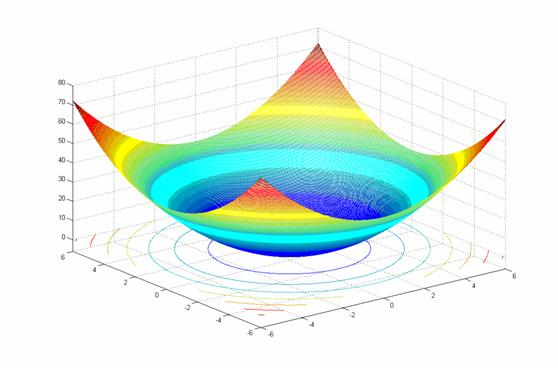
\includegraphics[height=150pt,keepaspectratio]{images/sphere-graph.jpg}
		\caption{Sphere function graph}
	\end{figure}

    
	\subsubsection{Dixon \& Price function}
	$$f(x_1 \cdots x_n) = (x_1 - 1)^2 ) + {\sum_{i=2}^{n} i(2x_i^{2} - x_{i-1})^2}, x_i \in [-10, 10]$$


	\begin{figure}[!h]
		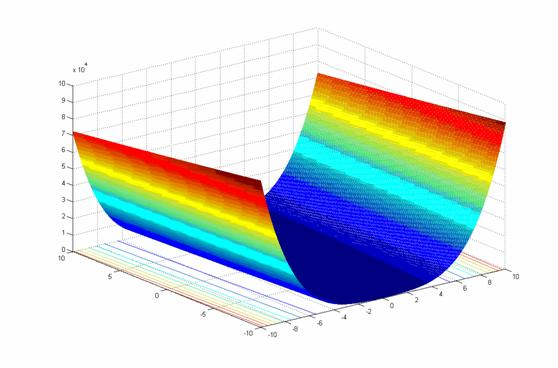
\includegraphics[height=150pt,keepaspectratio]{images/dixon-graph.jpg}
		\caption{Dixon \& Price function graph}
	\end{figure}

	\subsubsection{Michalewicz function}
	$$f(x_1 \cdots x_n) = -{\sum_{i=1}^{n} sin(x_i)\left[\frac{ix_i^2}{\pi}\right]^{2m}}, m = 10, x \in [0, \pi]$$

	\begin{figure}[!h]
		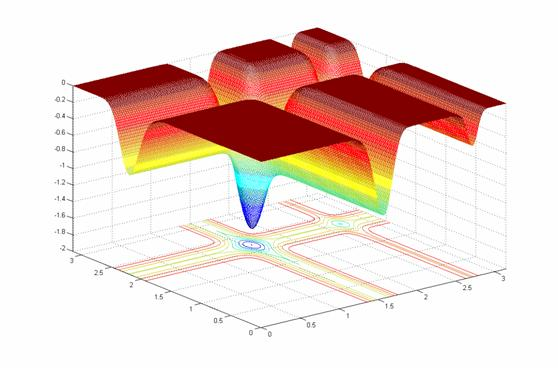
\includegraphics[height=150pt,keepaspectratio]{images/michalewicz-graph.jpg}
		\caption{Michalewicz function graph}
	\end{figure}

	\subsubsection{Rastrigin function}
	$$f(x_1 \cdots x_n) = 10n + \sum_{i=1}^n (x_i^2 -10cos(2\pi x_i)),$$

	\begin{figure}[!h]
		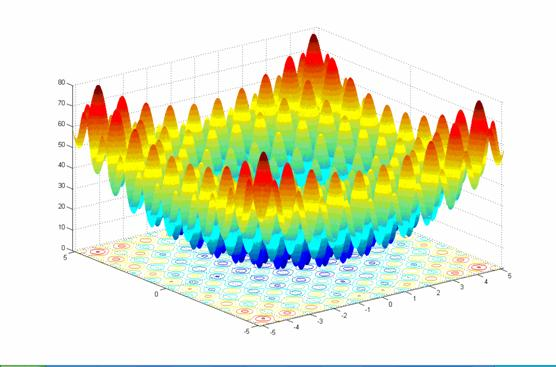
\includegraphics[height=150pt,keepaspectratio]{images/rastrigin-graph.jpg}
		\caption{Rastrigin function graph}
	\end{figure}
	
	\section{Experiment}
	For each of the four functions (for 2, 5 and 30 dimensions) the algorithm was run 30 times in parallel, each run limited to a time just above 600000ms (10 minutes). The results for each of the runs were transcribed in output files, which were then processed with a simple R script into a large \LaTeX\ table, which was then manually split, edited and spliced with the tables from last time. The results are below.
    \section{Results}
    \paragraph{}
    // todo: description

    \section{Result analysis}

    \section{References}
    \begin{itemize}
        \item Functions and graphs: \url{http://www-optima.amp.i.kyoto-u.ac.jp/member/student/hedar/Hedar_files/TestGO_files/Page364.htm}
    \end{itemize}


\end{document}
